\section{Improving Parameter Estimates by Solving Sequences of SIPs}\label{sec:mud-pde-sequence}
When progressing from two dimensions to five in the process of refining our estimate of $g$, we did so using an equal amount of parameter samples despite the volume of the spaces differing.
The measure of $\pspace$ (i.e., $\pmeas(\pspace)$), increased by a factor of $64$ while all else was held constant.
Too many of the functions considered by the initial density are impractical to consider because of their roughness.
In the linear examples of \ref{sec:high-dim-linear-example}, it is shown that initial densities which ascribe higher likelihood to the true parameter lead to MUD estimates that are more accurate.
By making better use of our model-evaluation budget of $1000$ samples for the PDE example, we find that both $\qoi_\text{1D}$ and $\qoi_\text{5D}$ perform significantly better in their ability to resolve $\paramref$.


%%%%%%%%%%%%%%%%%%%%%%%%%%%%%%%%%%%%%%%%%%%%%%%%%%%%%%%%%%%%%%%%
%%%%%%%%%%%%%%%%%%%%%%%%%%%%%%%%%%%%%%%%%%%%%%%%%%%%%%%%%%%%%%%%
\subsection{Motivations for a New Initial Density}
Reducing the volume of the support of the initial density will allow the samples drawn from it to better predict the collected data.
Recall from Example~\ref{subsec:pde-example} that two maps are used to solve the SIP: $\qoi_{1D}$ and $\qoi_{2D}$ and MUD points are shown for representative examples.
We use the solutions from those examples\---namely the ratio which updates the initial density\---to inform the construction of a new initial density in five dimensions.
In Figure~\ref{fig:pde-highd-2d-updated}, we plot the initial densities associated with $\qoi_{1D}$ and $\qoi_{2D}$ and remark that the scalar--valued QoI map identifies a contour which appears to trace a straight line through $\pspace$.
This is helpful for identifying the correlation structure and defining a lower-dimensional subspace to perform rejection sampling. However, the solution that comes from using $\qoi_{2D}$ is better at reducing uncertainty.
Taken together, these observations suggest a number of sampling strategies to generate a new initial density.

\begin{figure}
\centering
  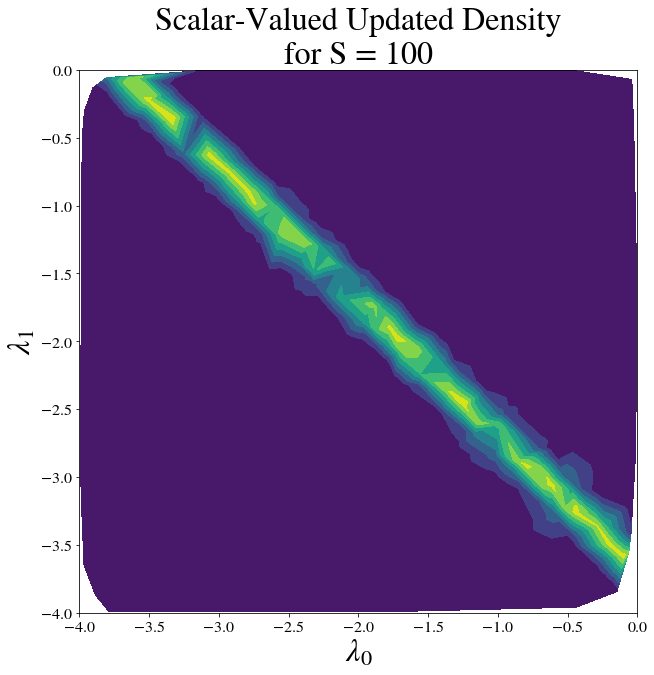
\includegraphics[width=0.45\linewidth]{figures/pde-highd/pde-highd_updated_D2_scalar.png}
  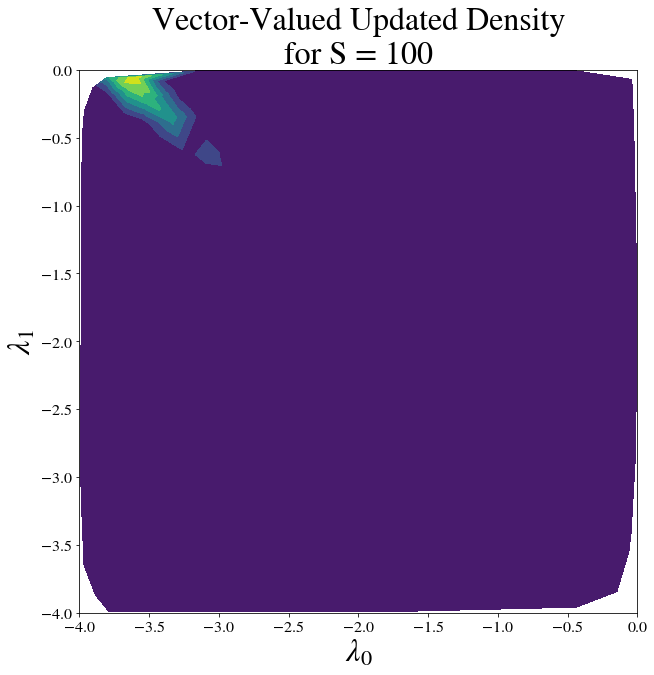
\includegraphics[width=0.45\linewidth]{figures/pde-highd/pde-highd_updated_D2_vector.png}
\caption{
100 measurements are used to solve the SIP for the PDE problem with $\qoi_{1D}$ and $\qoi_{2D}$.
}
\label{fig:pde-highd-2d-updated}
\end{figure}

By considering the relationship between the parameters and the types of functions that are possible given the solution to a 2-D inverse problem, we are able to create a more restricted parameter space in five dimensions.

For a detailed discussion of how a new initial density is constructed for this example, we refer the interested reader to Appendix~\ref{ext:pde-5d-initial}.
We summarize the procedure briefly:
First we generate uniform i.i.d. samples in the three dimensions associated with the new knot points by defining independent bounds for each and taking samples from the cross-product of the directions.\footnote{
The bounds for each are determined by looking at piecewise-linear estimates of $g$ that come from sampling the updated density for the vector--valued solution.
}
We generate $\nsamps=1000$ i.i.d. samples from this 2-D uniform density\footnote{
The (computational) cover is described by a procedure which involves the SVD of samples from the scalar--valued solutions in order to capture the correlation structure.
The use of the $\qoi_\text{1D}$ solution is due to the paucity of samples accepted from the vector--valued solution.
The structure of the latter updated density is more amenable to form a good estimate of this correlation direction in parameter space.
}
, and join them with the three other directions to form the new initial sample set, the functions from which generate the curves shown in Figure~\ref{fig:pde-highd-alt-initial-5d}.

\begin{figure}
\centering
  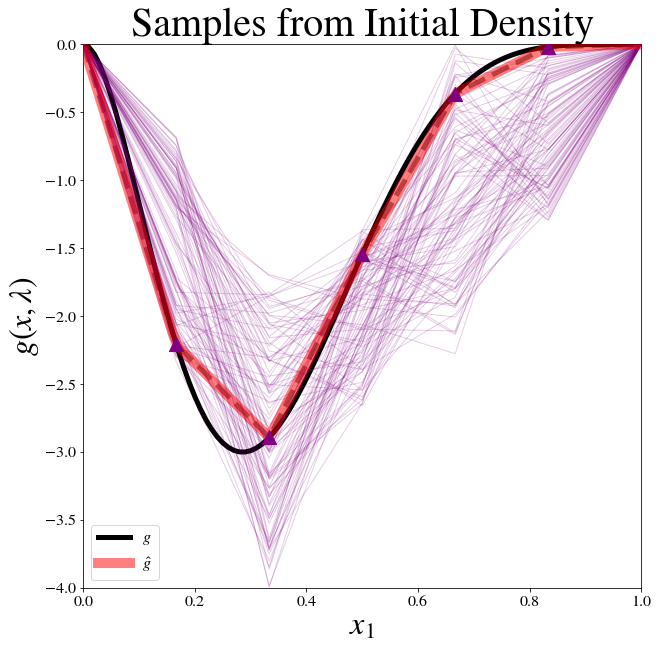
\includegraphics[width=0.675\linewidth]{figures/pde-highd/pde-highd_init_D5-alt}
\caption{
Initial density constructed for the second attempt at the five--dimensional inverse problem, with the structure of solutions learned from the 2-D example incorporated into the selection of bounds in each direction.
}
\label{fig:pde-highd-alt-initial-5d}
\end{figure}

The new initial curves in \ref{fig:pde-highd-alt-initial-5d}\---especially when contrasted to those in Fig.~\ref{fig:pde-highd-initial-5d}\---represent a far more reasonable set of possibilities.
The slope of the functions considered now all only have a single sign change, a marked improvement over the two or three that many samples from \ref{fig:pde-highd-initial-5d} exhibited.
We note that such considerations of smoothness could be avoided by parameterizing $g$ with a basis of some sort, but that problem is beyond the scope of this work.

%%%%%%%%%%%%%%%%%%%%%%%%%%%%%%%%%%%%%%%%%%%%%%%%%%%%%%%%%%%%%%%%
%%%%%%%%%%%%%%%%%%%%%%%%%%%%%%%%%%%%%%%%%%%%%%%%%%%%%%%%%%%%%%%%
\subsection{SIP Solutions using New Initial Density}
We now come to the solutions that arise from solving the same five--dimensional inverse problem of interpolating the values of $g$ through equispaced knot points, with both types of maps, in Figure~\ref{fig:pde-highd-5d-alt-mud}.
The difference in comparison to the solutions in Fig.~\ref{fig:pde-highd-5d-mud} is stark: no longer are the estimated functions dramatically under-estimating the local minimum of $g$.
The inadequacy of approximation error is attributable to the choice of knot points imposing a regular structure.
Since $g$'s minimum lies between two knot points, the best approximation of where this minimum is will by definition still be incorrect.

\begin{figure}
\centering
  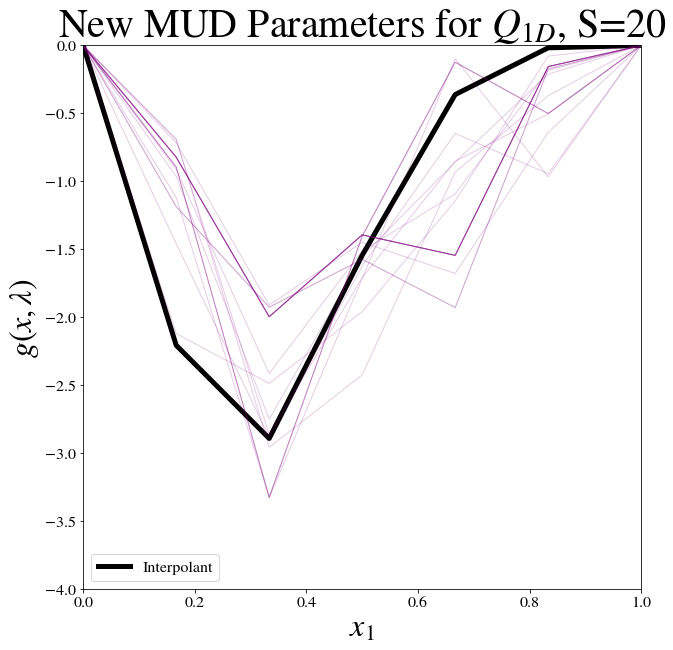
\includegraphics[width=0.45\linewidth]{figures/pde-highd/pde-highd_pair_D5-alt-5-1_m20.png}
  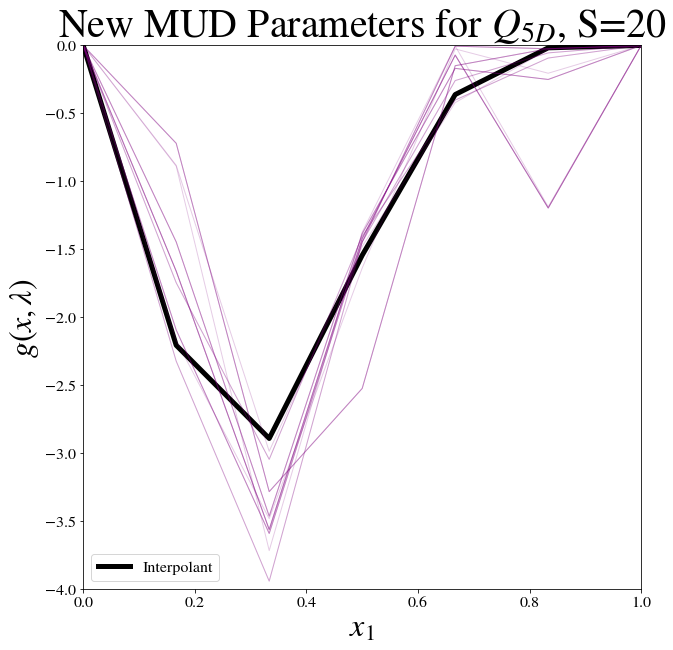
\includegraphics[width=0.45\linewidth]{figures/pde-highd/pde-highd_pair_D5-alt-5-5_m20.png}
  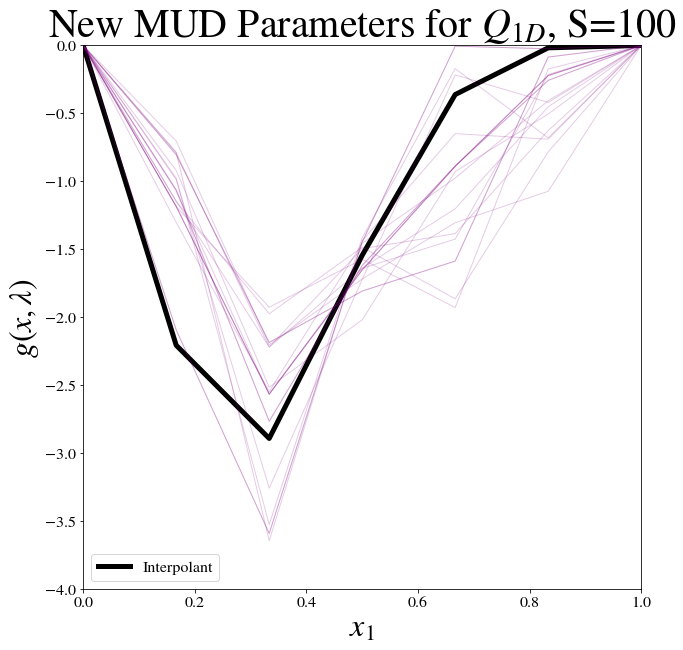
\includegraphics[width=0.45\linewidth]{figures/pde-highd/pde-highd_pair_D5-alt-5-1_m100.png}
  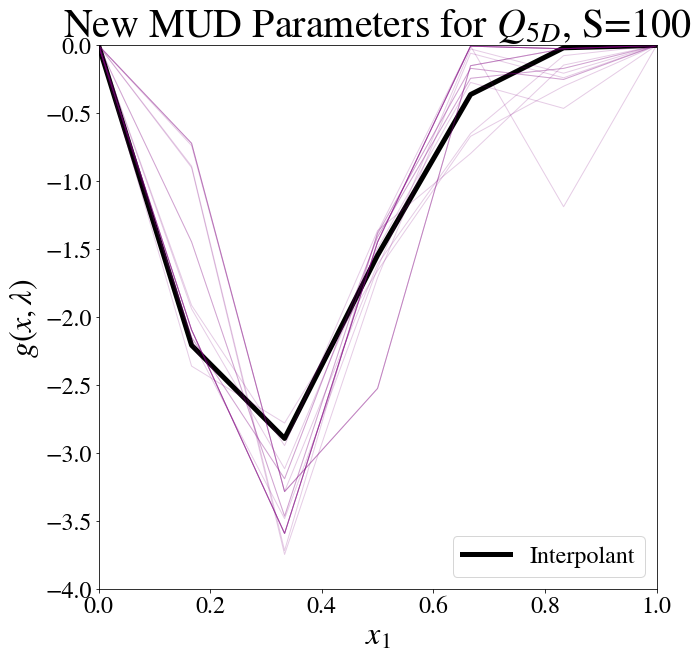
\includegraphics[width=0.45\linewidth]{figures/pde-highd/pde-highd_pair_D5-alt-5-5_m100.png}
\caption{Solutions to the SIP using one hundred measurements for $\ndata = 20$ (top) and $100$ (bottom).
(Left): Scalar-valued solutions for alternative approach to the five-dimensional problem.
(Right): Vector-valued solutions.
}
\label{fig:pde-highd-5d-alt-mud}
\end{figure}

Even when only $20$ measurements are incorporated into constructing the QoI maps, there is a considerable improvement in the predicted boundary conditions when using a better initial density, as seen by comparing the solutions in Fig.~\ref{fig:pde-highd-5d-alt-mud} to Fig.~\ref{fig:pde-highd-5d-mud}.
Owing to the reduced volume of support for the initial density, both QoI maps resolve the residuals similarly, especially as more data are incorporated (shown in the bottom of \ref{fig:pde-highd-5d-alt-mud}).
Since ``unreasonable'' functions are no longer being considered, both maps produce qualitatively similar estimates.

\subsection{Demonstration of Reduction in Uncertainty}
As a final note on this experiment, we contrast the resulting $L^2$-errors to $g$\footnote{derived from computational approximation with the trapezoidal rule} of these MUD solutions, to the previous two examples in Figure~\ref{fig:pde-highd-5d-hist}.
With each successive problem, our uncertainty is reduced and the MUD solutions have lower variance and improved accuracy.
Note that they appear to be moving towards a value away from zero, which represents a fixed bias (five equispaced knots can only approximate this particular $g$ so well).

\begin{figure}
\centering
  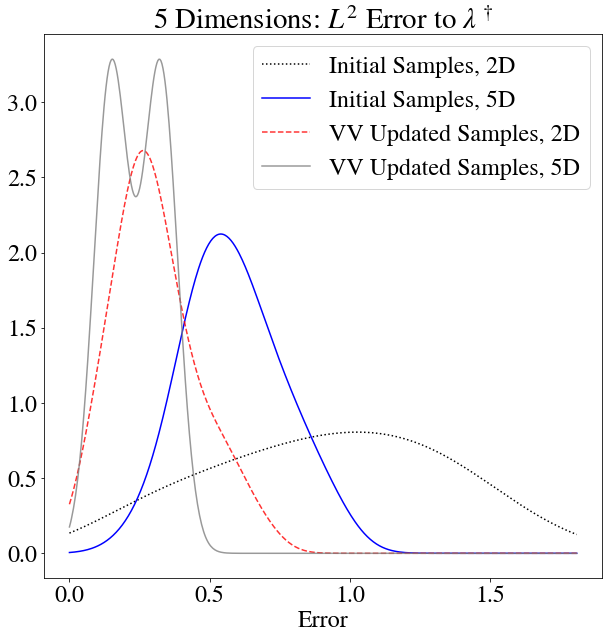
\includegraphics[width=0.675\linewidth]{figures/pde-highd/pde-highd_hist_D5_t5-0E-01}
\caption{
Comparison of the 2D initial errors to the 5D ones, as well as the reduction of uncertainty that solving a SIP problem for each provides.
}
\label{fig:pde-highd-5d-hist}
\end{figure}
